\section{Introduction}

% Reinforcement learning and it's uses
% Why we care about Multi-Goal Reinforcement Learning
Many tasks in robotics require the specification of a \emph{goal} for every
trial. For example, a robotic arm can be tasked to move an object to an arbitrary
goal position on a table \citep{gu2017deep}; a mobile robot can be
tasked to navigate to an arbitrary goal landmark on a map \citep{zhu2017target}. The
adaptation of reinforcement learning to such goal-conditioned tasks where goal
locations can change is called Multi-Goal Reinforcement Learning
(MGRL)~\citep{plappert2018multi}.
% A common way to solve MGRL problems is the use of Goal-Conditioned
% Value functions. Solving several tasks instead of individual tasks
State-of-the-art MGRL algorithms
\citep{andrychowicz2017hindsight, pong2018temporal}
work by estimating \emph{goal-conditioned value functions} (GCVF) which
are defined as expected cumulative rewards from 
start states with specified goals. GCVFs, in turn, are used to compute
\emph{policies} that determine the actions to take at every state.


% Goal conditioned value functions make a big assumption however. It is
% assumed that to learn to achieve goals, goal locations must themselves
% must be associated with reward. This however is not the case. We
% introduce ....
To learn GCVFs, MGRL algorithms use \emph{goal-reward},
defined as the relatively higher reward recieved on reaching the desired
goal state.
This makes the reward function dependent on the desired goal.
For example, in the Fetch-Push task \citep{plappert2018multi} of moving
a block to a given location on a table, every movement incurs a ``-1''
reward while reaching the desired goal returns a ``0'' goal-reward. 
This dependence introduces additional reward resampling steps in
algorithms like Hindsight Experience Replay (HER)
\citep{andrychowicz2017hindsight}, where
trials in which the agent failed to reach the goal are reused by recomputing
rewards as if the reached states were pseudo-desired goals.
Due to the dependence of the reward function on the goal,
the relabelling of every pseudo-goal requires an independent
\emph{reward-recomputation} step, which can be expensive. 

%This leads to the
%requirement of \emph{reward-recomputation}, which is that these reward functions can be
%computed indendent of \emph{environment} interaction.  The second assumption enables a technique called \emph{Hindsight
%Experience Replay} (HER) that accelerates learning 

% Do goal-conditioned value functions require goal rewards to learn?
% Describe some form of the intuition
%In this paper, we demonstrate that the goal-rewards requirement is
%avoidable. Let us consider an example to motivate why goal-rewards can
%be avoided in goal-conditioned tasks. Consider a student who has moved
%to a new university. To learn about the campus, the student explores it
%randomly with no specific goal in mind. The key intuition here is that
%the student is not incentivized to find specific goal locations (i.e.
%no goal rewards) but is aware of the effort required to travel between
%explored points around the university. When tasked with finding a
%goal classroom, the student can then use this learned path efforts to
%find least effort paths to the classroom. 
%
In this paper, we demonstrate that \emph{goal-rewards are not needed to
learn GCVFs}. For the Fetch-Push example, the ``0'' goal-reward does
not need to be achieved to learn its GCVF. Specifically, the agent
continues to receive ``-1'' reward even when the block is in the given
goal location. This reward formulation is atypical in conventional RL
because high reward is used to specify the desired goal location.
However, this goal-reward is not necessary in goal-conditioned RL because the
goal is already specified at the start of every episode.  We use this
idea, to propose a goal-conditioned RL algorithm which learns to reach
goals without goal-rewards. This is a counter-intuitive
result which is important for understanding goal-conditioned RL.

Let us consider another example to motivate the redundancy of goal-rewards.
Consider a student who has moved to a new campus. To learn about the campus,
the student explores it randomly with no specific goal in mind. The key
intuition here is that the student is not incentivized to find specific goal
locations (i.e. no goal-rewards) but is aware of the effort required to travel
between points around the university. When tasked with finding a goal classroom,
the student can chain together these path efforts to find the least-effort path
to the classroom.
%
Based on this intuition of least-effort paths, we redefine GCVFs to be
the expected \emph{path-reward} that is learned for all possible
start-goal pairs. We  
introduce a \emph{one-step loss} that assumes one-step paths 
to be the paths of maximum reward between pairs wherein the state and goal are adjacent.
Under this interpretation, the \emph{Bellman equation} chooses and chains
together one-step paths to find longer maximum reward paths. 
%
Experimentally, we show how this simple reinterpretation, which does not use goal
rewards, performs as well as HER while outperforming it in terms of
reward computation.

% Detail the Floyd-Warshall contribution
We also extend a closely related algorithm, Floyd-Warshall Reinforcement
Learning (FWRL) \citep{kaelbling1993learning} (also called Dynamic Goal
Reinforcement learning) to use parametric
function approximators instead of tabular functions. Similar to our
re-definition of GCVFs, FWRL learns a goal-conditioned Floyd-Warshall function
that represents path-rewards instead of future-rewards.
We translate FWRL's compositionality constraints in the space of GCVFs to introduce
additional loss terms to the objective. However, these additional loss
terms do not show improvement over the baseline. We conjecture that the
compositionality constraints are already captured by other loss terms. 

% Summarize 
In summary, the  contributions of this work are twofold. Firstly, we
reinterpret goal-conditioned value functions as expected path-rewards
and introduce one-step loss, thereby removing the dependency of GCVFs on
goal-rewards and reward resampling. We showcase our algorithm's
improved sample efficiency (in  terms of reward computation). We thus
extend algorithms like HER to domains where reward recomputation is
expensive or infeasible.
Secondly, we extend the tabular Floyd-Warshal Reinforcement Learning to
use deep neural networks. 

%% There is inherent structure in the formulation of these functions
%% thathas been ignored. Dhiman et al introduced structure in the space
%% of these functions 
%Floyd-Warshall Reinforcement Learning was first introduced in Dhiman et.
%al. for tabular domains. 
%The FW functions is defined 
%%
%\begin{align}
%\fwargs{\state}{\act}{\state'}{\policy}{} =
%\E_{\policy}\left[ \sum_{t=0}^{t=k} \rew_t \middle\vert \state_0 = \state, \act_0 = \state, \state_k = \state' \right] .
%\end{align}%
%%
%which is the expected sum of rewards when the state is s and the
%end state is the goal. Compositionality constraints are then used to
%learn the FW function.
%%
%\begin{align}
%\fwargs{\state_i}{\act_i}{\state_j}{\policy^*_{\state_j}}{*}
% \ge 
%  \fwargs{\state_i}{\act_i}{\state_k}{\policy^*_{\state_k}}{*}
%  + \max_{\act_k}\fwargs{\state_k}{\act_k}{\state_j}{\policy^*_{\state_j}}{*}
%  ,\forall \state_k \in \State.
%  \label{eq:fwconstraint}
%\end{align}%
%%
%The constraint is inspired by the Floyd-Warshall algorithm for path
%planning on graphs and states that the expected reward in traversing
%from one state to another should be greater than or equal to that of the
%paths through intermediary states.  While Dhiman et al. was restritcted
%to toy examples in the gridworld doman and tabular functions, they are
%not naturally scalabale to real life problems. This work extends their
%formulation to paramteric functions like neural networks by addition
%terms to the RL objective based on these compositionality constraints.
%Since we extend the algorithm to the Deep Learning domain, we call it
%Deep Floyd-Warshall Reinforcement Learning. 


%
\begin{figure}%
  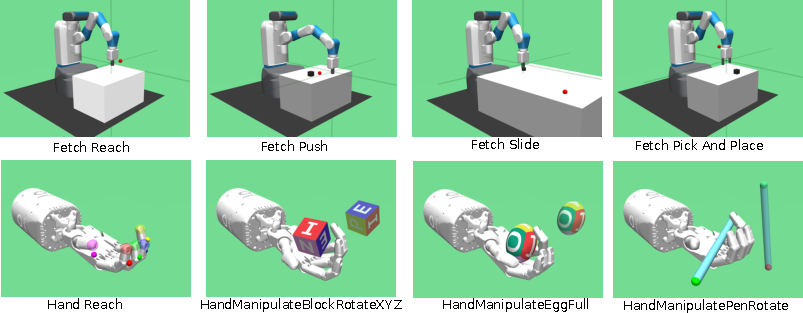
\includegraphics[width=\columnwidth]{./media/task-visuals-from-plappert.pdf}%
  \caption{\citet{plappert2018multi} introduce challenging tasks on the
Fetch robot and the Shadow Dextrous hand. We use these tasks for our experiments.
    Images are taken from the technical report.}%
  \label{fig:envs}%
\end{figure}%
% 
